\documentclass[11pt, a4paper]{article}\usepackage[]{graphicx}\usepackage[]{xcolor}
% maxwidth is the original width if it is less than linewidth
% otherwise use linewidth (to make sure the graphics do not exceed the margin)
\makeatletter
\def\maxwidth{ %
  \ifdim\Gin@nat@width>\linewidth
    \linewidth
  \else
    \Gin@nat@width
  \fi
}
\makeatother

\definecolor{fgcolor}{rgb}{0.345, 0.345, 0.345}
\newcommand{\hlnum}[1]{\textcolor[rgb]{0.686,0.059,0.569}{#1}}%
\newcommand{\hlsng}[1]{\textcolor[rgb]{0.192,0.494,0.8}{#1}}%
\newcommand{\hlcom}[1]{\textcolor[rgb]{0.678,0.584,0.686}{\textit{#1}}}%
\newcommand{\hlopt}[1]{\textcolor[rgb]{0,0,0}{#1}}%
\newcommand{\hldef}[1]{\textcolor[rgb]{0.345,0.345,0.345}{#1}}%
\newcommand{\hlkwa}[1]{\textcolor[rgb]{0.161,0.373,0.58}{\textbf{#1}}}%
\newcommand{\hlkwb}[1]{\textcolor[rgb]{0.69,0.353,0.396}{#1}}%
\newcommand{\hlkwc}[1]{\textcolor[rgb]{0.333,0.667,0.333}{#1}}%
\newcommand{\hlkwd}[1]{\textcolor[rgb]{0.737,0.353,0.396}{\textbf{#1}}}%
\let\hlipl\hlkwb

\usepackage{framed}
\makeatletter
\newenvironment{kframe}{%
 \def\at@end@of@kframe{}%
 \ifinner\ifhmode%
  \def\at@end@of@kframe{\end{minipage}}%
  \begin{minipage}{\columnwidth}%
 \fi\fi%
 \def\FrameCommand##1{\hskip\@totalleftmargin \hskip-\fboxsep
 \colorbox{shadecolor}{##1}\hskip-\fboxsep
     % There is no \\@totalrightmargin, so:
     \hskip-\linewidth \hskip-\@totalleftmargin \hskip\columnwidth}%
 \MakeFramed {\advance\hsize-\width
   \@totalleftmargin\z@ \linewidth\hsize
   \@setminipage}}%
 {\par\unskip\endMakeFramed%
 \at@end@of@kframe}
\makeatother

\definecolor{shadecolor}{rgb}{.97, .97, .97}
\definecolor{messagecolor}{rgb}{0, 0, 0}
\definecolor{warningcolor}{rgb}{1, 0, 1}
\definecolor{errorcolor}{rgb}{1, 0, 0}
\newenvironment{knitrout}{}{} % an empty environment to be redefined in TeX

\usepackage{alltt}

\usepackage[top=1 in, bottom = 1 in, left = 1 in, right = 1 in ]{geometry}

\usepackage{amsmath, amssymb, amsfonts}
\usepackage{enumerate}
\usepackage{array}
\usepackage{multirow}
\usepackage{dingbat}
\usepackage{fontawesome5}
\usepackage{tasks}
\usepackage{bbding}
\usepackage{xcolor}

\definecolor{col1}{HTML}{e75e05}
\definecolor{stack_red}{HTML}{DB4437}
\definecolor{stack_yellow}{HTML}{F4B400}
\definecolor{stack_cyan}{HTML}{08e2f0}
\definecolor{stack_blue}{HTML}{4285F4}
\definecolor{stack_green}{HTML}{0F9D58}

\title{MSMS - 105}
\author{Ananda Biswas}
\date{}
\IfFileExists{upquote.sty}{\usepackage{upquote}}{}
\begin{document}

\maketitle

\begin{center}
\textbf{Assignment 05}
\end{center}


\OrnamentDiamondSolid \hspace{0.5cm} \textcolor{blue}{\textbf{Objective :}} To create an animated plot that visually illustrates \textbf{Diffusion}. \\

\faArrowAltCircleRight[regular] \textcolor{col1}{\textbf{\textit{Theory}}} : Diffusion is the process by which molecules move from an area of higher concentration to an area of lower concentration, resulting in a uniform distribution of substances. This can occur in gases, liquids, and solids, and is driven by the random movement of particles. \\

\hspace{1cm} Diffusion is an everyday phenomenon. \\


\faArrowAltCircleRight[regular] \textcolor{col1}{\textbf{\textit{Code}}} : 

\begin{knitrout}\footnotesize
\definecolor{shadecolor}{rgb}{0.969, 0.969, 0.969}\color{fgcolor}\begin{kframe}
\begin{alltt}
\hldef{pause} \hlkwb{<-} \hlkwa{function}\hldef{(}\hlkwc{seconds}\hldef{)\{}
  \hldef{start} \hlkwb{<-} \hlkwd{Sys.time}\hldef{()}
  \hlkwa{while}\hldef{((}\hlkwd{Sys.time}\hldef{()} \hlopt{-} \hldef{start)} \hlopt{<} \hldef{seconds)\{\}}
\hldef{\}}
\end{alltt}
\end{kframe}
\end{knitrout}

\begin{knitrout}\footnotesize
\definecolor{shadecolor}{rgb}{0.969, 0.969, 0.969}\color{fgcolor}\begin{kframe}
\begin{alltt}
\hldef{diffusion} \hlkwb{<-} \hlkwa{function}\hldef{()\{}
  \hlkwd{par}\hldef{(}\hlkwc{bg} \hldef{=} \hlsng{"black"}\hldef{)}

  \hlkwa{for}\hldef{(i} \hlkwa{in} \hlkwd{seq}\hldef{(}\hlnum{0.1}\hldef{,} \hlnum{1}\hldef{,} \hlnum{0.1}\hldef{))\{}

    \hlkwd{plot}\hldef{(}\hlnum{NA}\hldef{,} \hlnum{NA}\hldef{,}
         \hlkwc{xlim} \hldef{=} \hlkwd{c}\hldef{(}\hlopt{-}\hlnum{1}\hldef{,} \hlnum{1}\hldef{),}
         \hlkwc{ylim} \hldef{=} \hlkwd{c}\hldef{(}\hlopt{-}\hlnum{1}\hldef{,} \hlnum{1}\hldef{))}

    \hldef{x} \hlkwb{<-} \hlkwd{runif}\hldef{(}\hlnum{400}\hldef{,} \hlopt{-}\hlnum{1.3}\hldef{,} \hlnum{1.3}\hldef{); y} \hlkwb{<-} \hlkwd{runif}\hldef{(}\hlnum{400}\hldef{,} \hlopt{-}\hlnum{1.3}\hldef{,} \hlnum{1.3}\hldef{)}

    \hlkwd{points}\hldef{(x, y,} \hlkwc{col} \hldef{=} \hlsng{"green"}\hldef{)}

    \hlkwd{pause}\hldef{(}\hlnum{0.35}\hldef{)}
  \hldef{\}}

  \hlkwa{for}\hldef{(i} \hlkwa{in} \hlkwd{seq}\hldef{(}\hlnum{0.1}\hldef{,} \hlnum{1}\hldef{,} \hlnum{0.1}\hldef{))\{}

    \hlkwd{plot}\hldef{(}\hlnum{NA}\hldef{,} \hlnum{NA}\hldef{,}
         \hlkwc{xlim} \hldef{=} \hlkwd{c}\hldef{(}\hlopt{-}\hlnum{1}\hldef{,} \hlnum{1}\hldef{),}
         \hlkwc{ylim} \hldef{=} \hlkwd{c}\hldef{(}\hlopt{-}\hlnum{1}\hldef{,} \hlnum{1}\hldef{))}

    \hldef{x} \hlkwb{<-} \hlkwd{runif}\hldef{(}\hlnum{400}\hldef{,} \hlopt{-}\hlnum{1.3}\hldef{,} \hlnum{1.3}\hldef{); y} \hlkwb{<-} \hlkwd{runif}\hldef{(}\hlnum{400}\hldef{,} \hlopt{-}\hlnum{1.3}\hldef{,} \hlnum{1.3}\hldef{)}

    \hldef{x1} \hlkwb{<-} \hlkwd{rnorm}\hldef{(}\hlnum{100}\hldef{,} \hlnum{0}\hldef{, i); y1} \hlkwb{<-} \hlkwd{rnorm}\hldef{(}\hlnum{100}\hldef{,} \hlnum{0}\hldef{, i)}

    \hlkwd{points}\hldef{(x, y,} \hlkwc{col} \hldef{=} \hlsng{"green"}\hldef{)}

    \hlkwd{points}\hldef{(x1, y1,} \hlkwc{col} \hldef{=} \hlsng{"red"}\hldef{,} \hlkwc{pch} \hldef{=} \hlnum{19}\hldef{)}

    \hlkwd{pause}\hldef{(}\hlnum{1}\hldef{)}
  \hldef{\}}
\hldef{\}}
\end{alltt}
\end{kframe}
\end{knitrout}

\begin{knitrout}
\definecolor{shadecolor}{rgb}{0.969, 0.969, 0.969}\color{fgcolor}\begin{kframe}
\begin{alltt}
\hlkwd{diffusion}\hldef{()}
\end{alltt}
\end{kframe}
\end{knitrout}



\faArrowAltCircleRight[regular] \textcolor{col1}{\textbf{\textit{Visualization}}} : Suppose we have a container filled with gas. Its molecules make movements randomly (shown by \textcolor{green}{Green} dots).

\begin{table}[!htbp]

\begin{center}
\begin{tabular}{ccc}

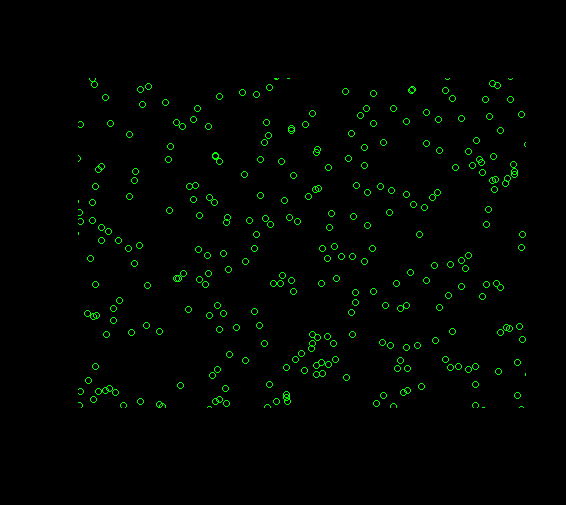
\includegraphics[scale = 0.35]{00} & 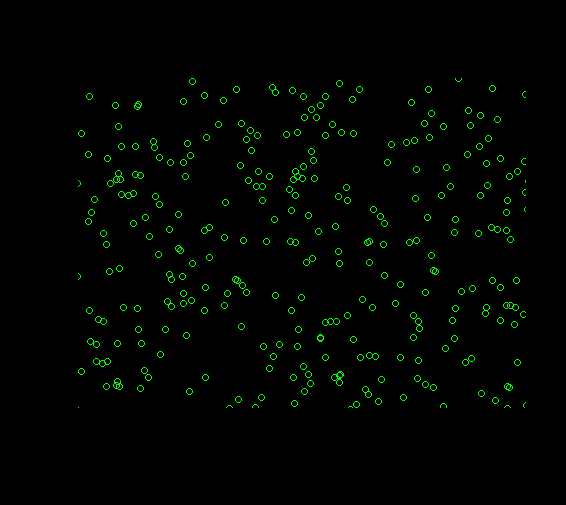
\includegraphics[scale = 0.35]{01} & 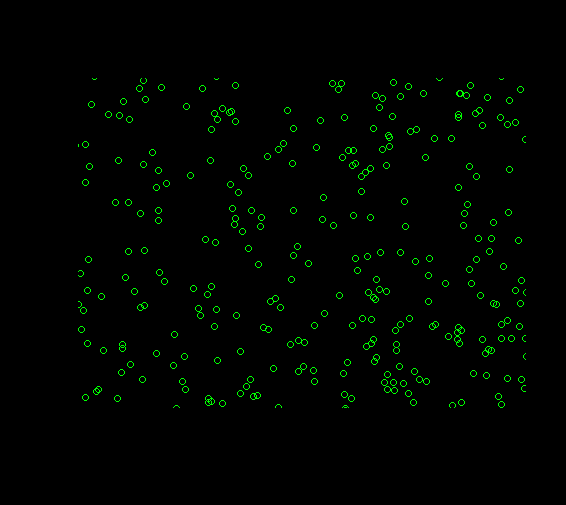
\includegraphics[scale = 0.35]{02}\\

\end{tabular}
\end{center}
\end{table}

A pocket of another gas (shown by \textcolor{red}{Red} dots) is dropped in the container and it gets mixed with the gas in the container uniformly over time.

\begin{table}[!htbp]

\begin{center}
\begin{tabular}{ccc}

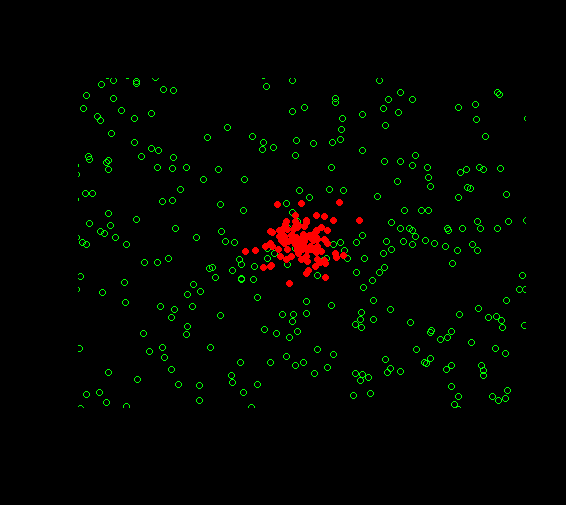
\includegraphics[scale = 0.35]{03} & 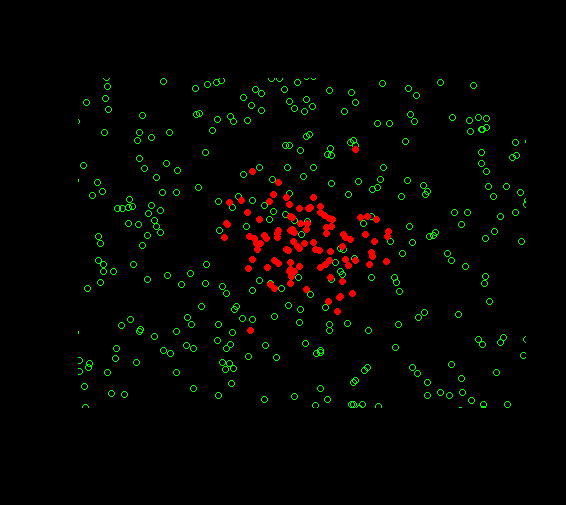
\includegraphics[scale = 0.35]{04} & 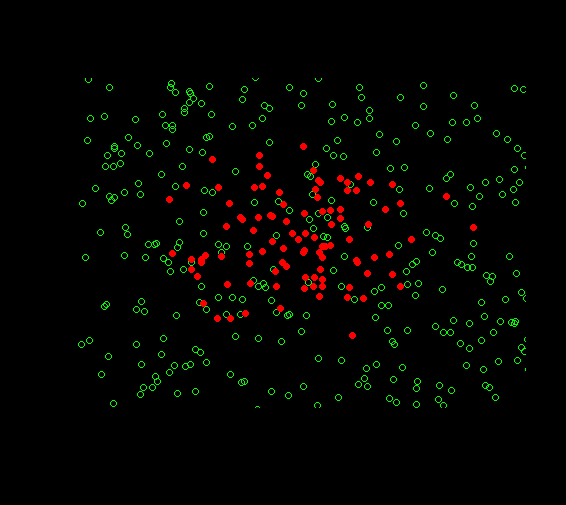
\includegraphics[scale = 0.35]{05} \\

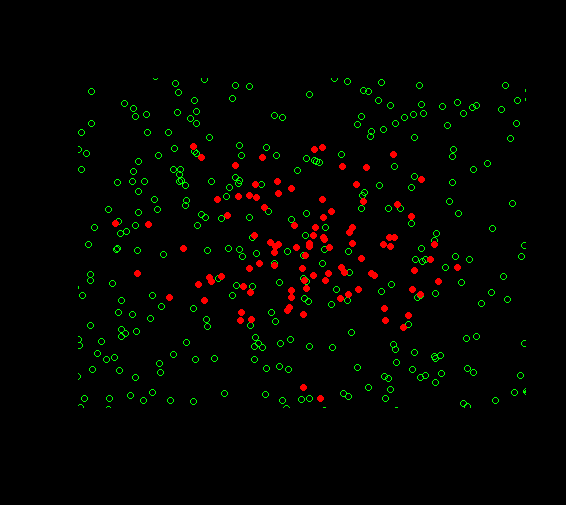
\includegraphics[scale = 0.35]{06} & 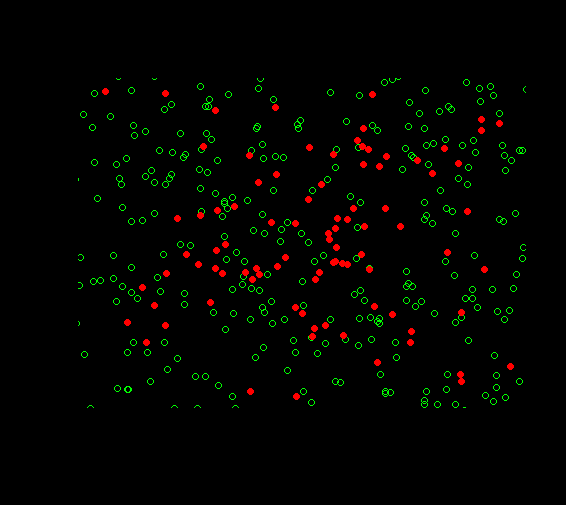
\includegraphics[scale = 0.35]{07} & 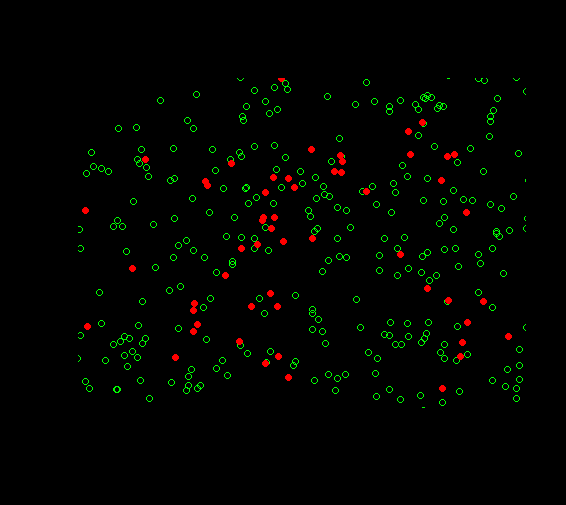
\includegraphics[scale = 0.35]{08} \\

\end{tabular}
\end{center}
\end{table}

\end{document}
